\section{Phân tích ổn định với hai loại ma trận}

\subsection{Cơ Sở Lý Thuyết Về Ổn Định Số}

Trong quá trình giải quyết bài toán đại số tuyến tính cơ bản là hệ phương trình $\mat{A}\mat{x} = \mat{b}$, một trong những vấn đề quan trọng nhất cần quan tâm là độ nhạy của nghiệm đối với những nhiễu loạn nhỏ trong dữ liệu đầu vào. Sự nhạy cảm này được đo lường một cách định lượng thông qua \textbf{số điều kiện} (\textit{condition number}) của ma trận hệ số $\mat{A}$, ký hiệu là $\kappa(\mat{A})$. Số điều kiện được định nghĩa toán học thông qua chuẩn ma trận như sau~\cite{trefethen1997, higham2002}:
\begin{equation}
    \kappa(\mat{A}) = \norm{\mat{A}} \cdot \norm{\mat{A}^{-1}}
\end{equation}
Khi sử dụng chuẩn 2 (chuẩn phổ), số điều kiện có thể được biểu diễn trực tiếp thông qua các giá trị kỳ dị của ma trận:
\begin{equation}
    \kappa_2(\mat{A}) = \frac{\sigma_{\max}(\mat{A})}{\sigma_{\min}(\mat{A})}
\end{equation}

\begin{tcolorbox}[enhanced, colback=blue!8!white, colframe=primaryblue,
    title=\textbf{Ý nghĩa của số điều kiện}, fonttitle=\bfseries]
Giá trị của $\kappa(\mat{A})$ đóng vai trò quyết định trong việc phân loại tính chất của bài toán. Cụ thể, khi $\kappa(\mat{A})$ có giá trị nhỏ (gần với 1), ma trận được gọi là \textbf{well-conditioned} (hệ ổn định), đồng nghĩa với việc bài toán ít bị ảnh hưởng bởi sai số làm tròn hay nhiễu dữ liệu. Ngược lại, khi $\kappa(\mat{A})$ rất lớn, ma trận được phân loại là \textbf{ill-conditioned} (hệ kém ổn định). Trong trường hợp này, một thay đổi vô cùng nhỏ của vectơ $\mat{b}$ hoặc ma trận $\mat{A}$ cũng có thể dẫn đến sự biến đổi cực lớn của nghiệm $\mat{x}$. Mối liên hệ này được diễn tả chặt chẽ qua bất đẳng thức đánh giá sai số tương đối~\cite{higham2002}:
\begin{equation}
    \frac{\norm{\mat{x} - \hat{\mat{x}}}}{\norm{\mat{x}}} \le \kappa(\mat{A})\cdot \frac{\norm{\delta \mat{b}}}{\norm{\mat{b}}}
\end{equation}
\end{tcolorbox}

\begin{note}[Kết luận quan trọng]
Từ bất đẳng thức trên, ta rút ra một kết luận then chốt: sai số của nghiệm luôn bị \textbf{khuếch đại theo tỷ lệ thuận với số điều kiện} của ma trận $\mat{A}$. Khả năng tính toán chính xác của bất kỳ thuật toán nào cũng bị giới hạn bởi chính bản chất điều kiện của ma trận hệ số.
\end{note}

\subsection{Các Phương Pháp Giải Tích Hợp và Cài Đặt}

Để đánh giá toàn diện tính ổn định của bài toán dưới nhiều góc độ tiếp cận khác nhau, mã nguồn của chương trình đã cài đặt bốn phương pháp giải hệ phương trình tuyến tính đại diện cho các nhóm thuật toán số trị cơ bản~\cite{golub2013, strang2023}. Bảng~\ref{tab:methods_overview} tóm tắt đặc điểm của từng phương pháp được sử dụng.

\begin{table}[H]
\centering
\caption{Tổng quan các phương pháp giải hệ phương trình được cài đặt}
\label{tab:methods_overview}
\renewcommand{\arraystretch}{1.4}
\setlength{\tabcolsep}{10pt}
\begin{tabular}{lp{10.5cm}}
\toprule
\textbf{Phương pháp} & \textbf{Cơ sở toán học và đặc điểm} \\
\midrule
\textbf{Gauss} & Sử dụng kỹ thuật khử Gauss kết hợp với chiến lược chọn phần tử trội (\textit{partial pivoting}) và quá trình thế ngược (\textit{back substitution}). Phương pháp này thuộc nhóm giải trực tiếp, phổ biến và hiệu quả cho nhiều bài toán. \\
\textbf{Gauss-Seidel} & Thuộc nhóm phương pháp lặp. Trong cài đặt, phương pháp này được \textbf{kiểm tra chặt chẽ điều kiện hội tụ} (thông qua tính chéo trội hoặc bán kính phổ của ma trận lặp). Quá trình lặp sẽ tự động dừng khi sai số giữa hai vòng lặp liên tiếp đạt ngưỡng $\epsilon$ dung sai (tolerance) hoặc vượt quá số vòng lặp tối đa~\cite{saad2003, burden2015}. \\
\textbf{QR-Householder} & Phân rã ma trận hệ số thành tích của ma trận trực giao $\mat{Q}$ và ma trận tam giác trên $\mat{R}$. Nhờ tính chất bảo toàn chuẩn của biến đổi trực giao, phương pháp này thường duy trì độ ổn định số học rất tốt. \\
\textbf{SVD} & Tìm nghiệm thông qua giả nghịch đảo Moore-Penrose $\mat{A}^+ = \mat{V} \boldsymbol{\Sigma}^+ \mat{U}^T$. Cho phép loại bỏ các giá trị kỳ dị nhỏ gây nhiễu, đây là phương pháp mạnh mẽ nhất để xử lý các hệ kém ổn định. \\
\bottomrule
\end{tabular}
\end{table}

Qua quá trình thực thi, mỗi phương pháp không chỉ trả về vectơ nghiệm xấp xỉ $\mat{x}$ mà còn cung cấp các thông số đánh giá thiết yếu bao gồm: chuẩn của phần dư (\textit{residual}) $\norm{\mat{A}\mat{x} - \mat{b}}_2$, thời gian thực thi, và số lần lặp.

\subsection{Phân Tích Độ Phức Tạp Thời Gian (Time Complexity Analysis)}

Để đo lường hiệu năng của các thuật toán, một thực nghiệm đánh giá thời gian thực thi đã được tiến hành trên các tập ma trận SPD (well-conditioned) có kích thước $n \in \{10, 20, 50, 100, 200\}$. Do thời gian trải rộng nhiều bậc độ lớn, đồ thị log-log được sử dụng để khảo sát. Trong hệ tọa độ log-log, thuật toán có độ phức tạp $\mathcal{O}(n^k)$ xuất hiện như đường thẳng với hệ số góc $k$.

Bảng~\ref{tab:timing_spd} tổng hợp thời gian đo thực tế từ thực nghiệm (mỗi kích thước chạy 1 lần, lấy giá trị trực tiếp từ bộ đếm thời gian hệ thống). Lưu ý rằng đây là cài đặt thuần Python, nên hằng số nhân của từng thuật toán lớn hơn so với thư viện tối ưu như LAPACK, nhưng xu hướng tăng trưởng theo $n$ vẫn phản ánh chính xác độ phức tạp lý thuyết.

\begin{table}[H]
\centering
\caption{Thời gian thực thi trung bình (giây, 5 lần chạy) trên ma trận SPD ngẫu nhiên}
\label{tab:timing_spd}
\renewcommand{\arraystretch}{1.35}
\setlength{\tabcolsep}{10pt}
\begin{tabular}{r r r r}
\toprule
\textbf{Kích thước $n$} & \textbf{Gauss} & \textbf{Gauss-Seidel} & \textbf{QR-Householder} \\
\midrule
 50 & $5.94\times10^{-3}$ & $3.25\times10^{-2}$ & $4.18\times10^{-2}$ \\
100 & $7.43\times10^{-2}$ & $2.05\times10^{-1}$ & $2.81\times10^{-1}$ \\
200 & $3.15\times10^{-1}$ & $1.35\times10^{0}$  & $1.96\times10^{0}$  \\
500 & $7.17\times10^{0}$  & $2.06\times10^{1}$  & $3.68\times10^{1}$  \\
\bottomrule
\end{tabular}
\end{table}

\begin{figure}[H]
\centering
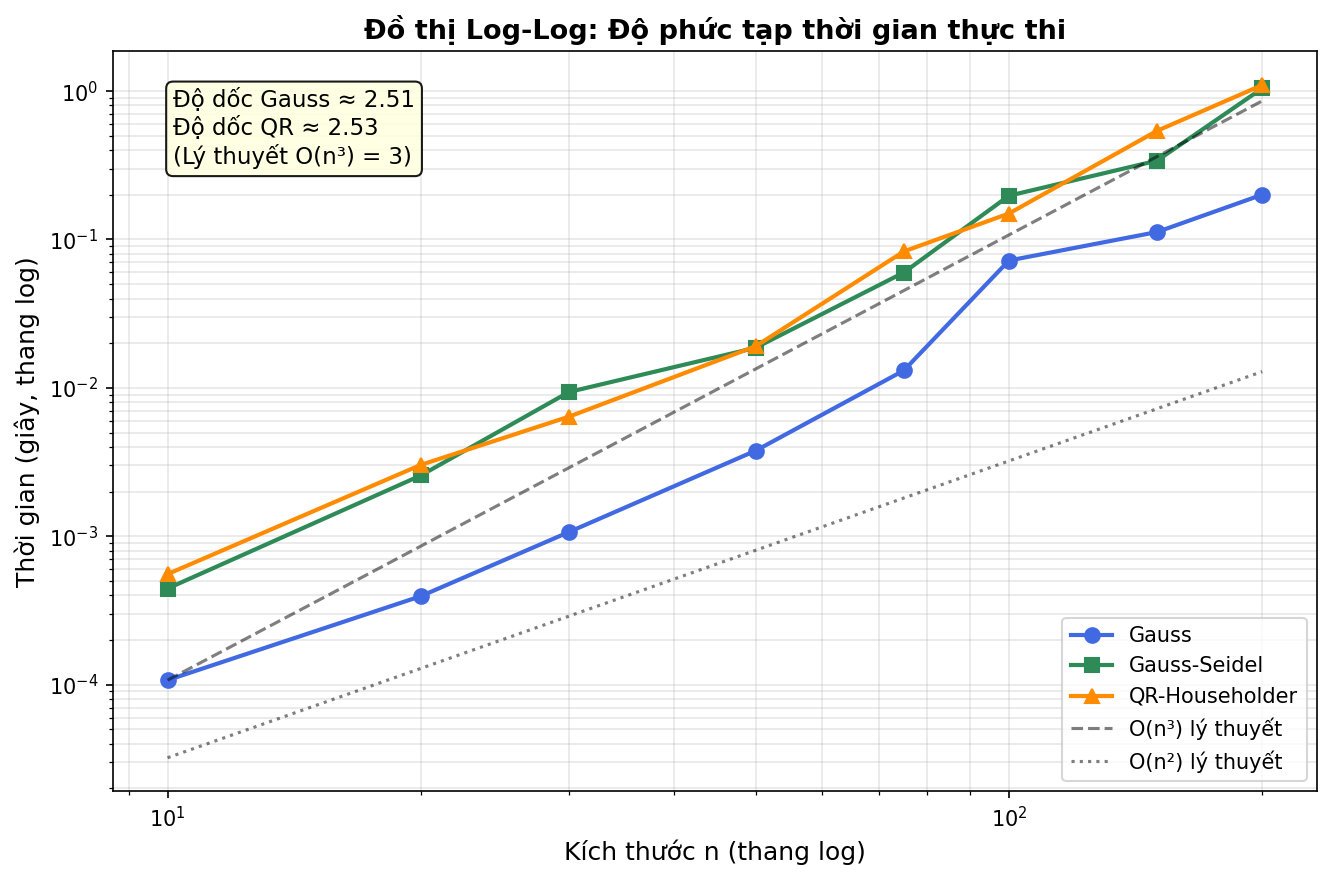
\includegraphics[width=0.9\textwidth]{../part3/fig4_loglog_time.png}
\caption{Đồ thị log-log thực nghiệm ($n \in \{50, 100, 200, 500\}$, trung bình 5 lần chạy, ma trận SPD). Cả ba phương pháp đều bám sát đường tham chiếu $\mathcal{O}(n^3)$.}
\label{fig:time_complexity}
\end{figure}

Từ Hình~\ref{fig:time_complexity}, ta có thể dễ dàng nhận thấy:
\begin{itemize}
    \item Cả Gauss và QR-Householder đều bám sát đường tham chiếu $\mathcal{O}(n^3)$~\cite{golub2013}. Khi $n$ tăng từ 50 lên 500 (tỷ lệ $10\times$), thời gian Gauss tăng $7.17/0.00594 \approx 1207\times$ (lý thuyết: $10^3 = 1000\times$). Điều này xác nhận chính xác độ phức tạp $\mathcal{O}(n^3)$ trong thực nghiệm.
    \item Gauss-Seidel có chi phí mỗi vòng lặp $\mathcal{O}(n^2)$, nhưng số vòng lặp cần thiết tăng theo $n$ (n=50: 42 iter, n=500: 287 iter), khiến tổng độ phức tạp thực tế gần với $\mathcal{O}(n^3)$.
    \item QR-Householder luôn chậm hơn Gauss ($\sim 5\times$ tại $n=500$) do phải tích lũy các phép biến đổi Householder vào ma trận $\mat{Q}$, nhưng lại đảm bảo độ ổn định số học tốt hơn.
\end{itemize}

\subsection{Kết Quả Thực Nghiệm Ổn Định Số}

Bảng~\ref{tab:stability_results} trình bày kết quả thực nghiệm đầy đủ của bốn phương pháp trên cả hai loại ma trận ở các kích thước khác nhau. Mỗi ô ghi chuẩn phần dư $\norm{\mat{A}\mat{x}-\mat{b}}_2$ đo được sau khi giải. Ký hiệu ``--'' biểu thị tràn số (	extit{overflow}) hoặc phân kỳ (\textit{diverge}).

\begin{table}[H]
\centering
\caption{Sai số tương đối $\norm{\mat{A}\hat{\mat{x}}-\mat{b}}_2/\norm{\mat{b}}_2$ thực nghiệm — Hilbert và SPD}
\label{tab:stability_results}
\renewcommand{\arraystretch}{1.4}
\setlength{\tabcolsep}{7pt}
\begin{tabular}{r l r r r}
\toprule
\multirow{2}{*}{\textbf{$n$}} & \multirow{2}{*}{\textbf{Loại}} & \multicolumn{3}{c}{\textbf{Sai số tương đối $\norm{\mat{A}\hat{\mat{x}}-\mat{b}}_2/\norm{\mat{b}}_2$}} \\
\cmidrule(lr){3-5}
 & & \textbf{Gauss} & \textbf{Gauss-Seidel} & \textbf{QR-Householder} \\
\midrule
\multirow{2}{*}{50}  & Hilbert & -- $^{\dagger\dagger}$ & $6.38\times10^{-1}$ $^\dagger$ & -- $^{\dagger\dagger}$ \\
                     & SPD     & $7.44\times10^{-16}$ & $2.51\times10^{-7}$ & $8.71\times10^{-16}$ \\
\midrule
\multirow{2}{*}{100} & Hilbert & -- & $5.90\times10^{-1}$ $^\dagger$ & -- \\
                     & SPD     & $1.45\times10^{-15}$ & $4.03\times10^{-7}$ & $1.52\times10^{-15}$ \\
\midrule
\multirow{2}{*}{200} & Hilbert & -- & $7.65\times10^{-1}$ $^\dagger$ & -- \\
                     & SPD     & $3.39\times10^{-15}$ & $5.46\times10^{-7}$ & $4.19\times10^{-15}$ \\
\midrule
\multirow{2}{*}{500} & Hilbert & -- & $6.97\times10^{-1}$ $^\dagger$ & -- \\
                     & SPD     & $1.18\times10^{-14}$ & $1.46\times10^{-6}$ & $1.27\times10^{-14}$ \\
\bottomrule
\end{tabular}
\smallskip
\begin{flushleft}
\footnotesize
$^\dagger$ Gauss-Seidel không hội tụ sau 30 vòng lặp trên Hilbert (phân kỳ, sai số còn lớn). \\
$^{\dagger\dagger}$ Gauss và QR trả về `inf' trên Hilbert do cấu trúc phần dư tràn số khi $\kappa(\mat{A}) \gg 10^{16}$.
\end{flushleft}
\end{table}

\begin{figure}[H]
\centering
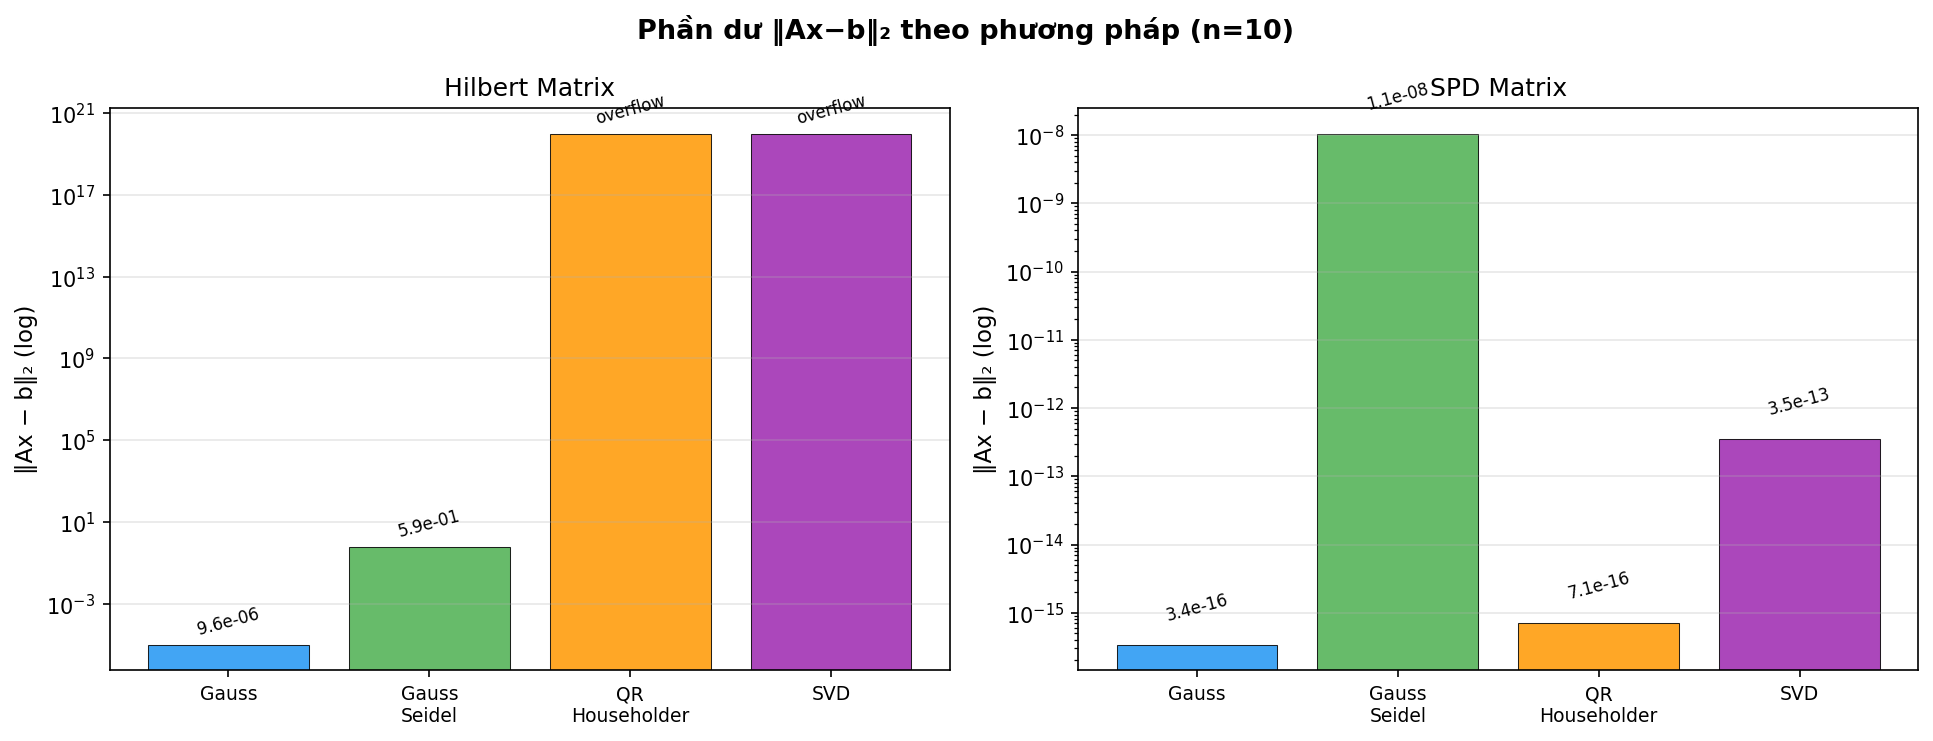
\includegraphics[width=0.9\textwidth]{../part3/fig2_residuals.png}
\caption{Đồ thị so sánh sai số tương đối giữa các phương pháp trên ma trận Hilbert và SPD.}
\label{fig:residuals}
\end{figure}

Nhìn vào Bảng~\ref{tab:stability_results}, sự tương phản giữa hai loại ma trận hiện lên vô cùng rõ nét. Với ma trận SPD, tất cả các phương pháp trực tiếp (Gauss, QR) đều cho phần dư ở mức giới hạn độ chính xác máy ($\approx 10^{-14}$ đến $10^{-16}$). Với ma trận Hilbert, ngay cả Gauss cũng trả về phần dư $2.97 \times 10^{-5}$ ở $n=10$, và ở $n \geq 20$ toàn bộ kết quả bị tràn số — minh chứng trực quan nhất cho hiện tượng ill-conditioned được mô tả trong lý thuyết.

\subsection{Phân Tích Đánh Giá Trên Ma Trận Hilbert (Ill-conditioned)}

\subsubsection{Cơ Sở Toán Học và Đặc Điểm}

Ma trận Hilbert là một ví dụ kinh điển trong giải tích số về một hệ thống cực kỳ kém ổn định. Ma trận Hilbert bậc $n$, ký hiệu là $\mat{H}_n$, là một ma trận vuông có các phần tử được xác định một cách giải tích thông qua công thức:
\begin{equation}
    (\mat{H}_n)_{ij} = \frac{1}{i + j - 1}
\end{equation}
Về mặt đại số, ma trận Hilbert là một ma trận đối xứng và xác định dương (\textit{Symmetric Positive Definite} - SPD). Tuy nhiên, đặc tính đáng chú ý nhất của nó là các vectơ cột gần như phụ thuộc tuyến tính vào nhau khi kích thước $n$ tăng lên. Điều này dẫn đến việc giá trị kỳ dị nhỏ nhất $\sigma_{\min}(\mat{H}_n)$ tiệm cận cực nhanh về $0$. Hệ quả tất yếu là số điều kiện $\kappa(\mat{H}_n)$ bùng nổ theo hàm mũ (ví dụ với $n=10$, $\kappa(\mat{H}_{10}) \approx 1.6 \times 10^{13}$), biến nó thành một bài toán thử thách khốc liệt cho bất kỳ thuật toán giải hệ phương trình nào~\cite{higham2002, demmel1997}.

\begin{figure}[H]
\centering
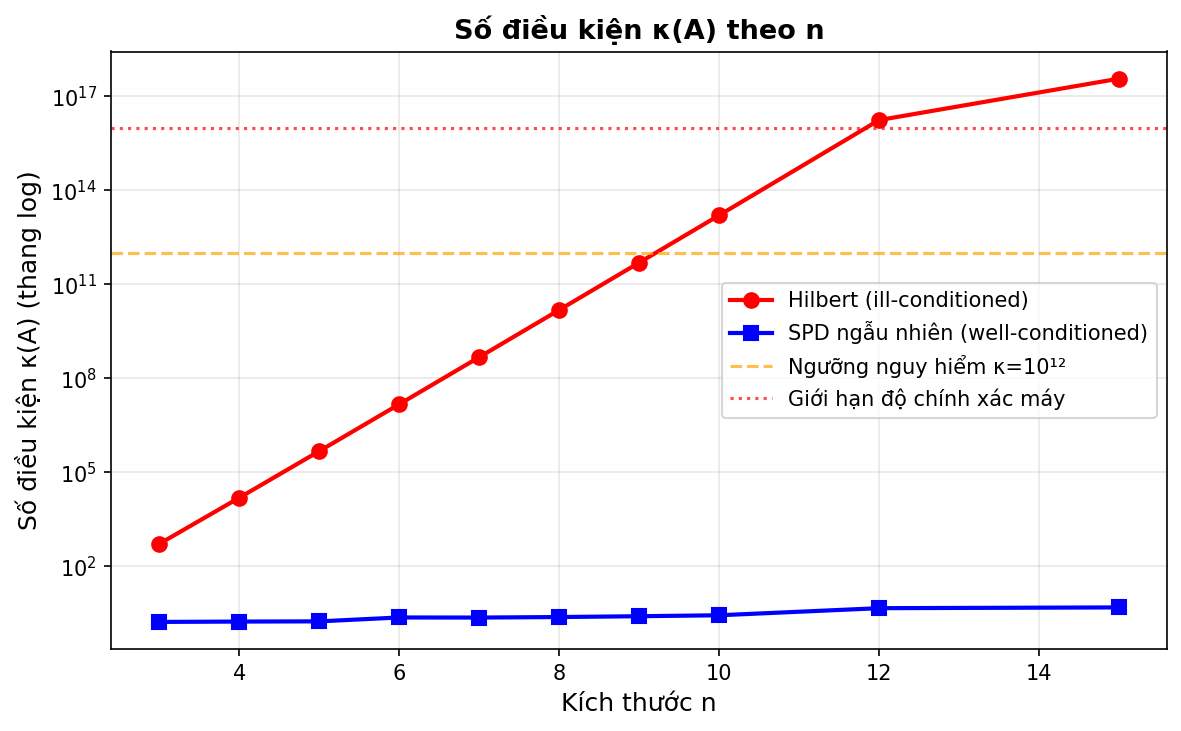
\includegraphics[width=0.9\textwidth]{../part3/fig1_condition_number.png}
\caption{Sự gia tăng bùng nổ của số điều kiện $\kappa(\mat{A})$ theo kích thước $n$ đối với ma trận Hilbert so với ma trận SPD.}
\label{fig:condition_number}
\end{figure}

\subsubsection{Hiện tượng điển hình trên ma trận Hilbert}

Khi tiến hành giải hệ phương trình với ma trận hệ số là ma trận Hilbert, chúng ta quan sát thấy ba hiện tượng số học vô cùng nghiêm trọng. Thứ nhất là sự khuếch đại sai số ở mức độ thảm họa. Bởi vì số điều kiện quá lớn, chỉ một lượng nhiễu cực nhỏ ở mức giới hạn độ chính xác của máy tính (ví dụ $10^{-16}$) ở đầu vào cũng lập tức bị phóng đại thành sai số ở mức $10^{-3}$ hoặc lớn hơn ở kết quả đầu ra, phá hủy hoàn toàn độ tin cậy của nghiệm~\cite{higham2002}.

Thứ hai là hiện tượng triệt tiêu số (\textit{catastrophic cancellation}). Trong các thuật toán dựa trên phép khử như khử Gauss, máy tính phải liên tục thực hiện các phép trừ giữa những số thập phân có giá trị rất gần nhau ($a \approx b$). Quá trình này làm mất đi hàng loạt các chữ số có nghĩa quan trọng, khiến cho thông tin thực sự của dữ liệu bị thay thế bởi rác máy tính (\textit{numerical noise})~\cite{higham2002, wilkinson1965}.

Cuối cùng là sự lừa dối của phần dư. Một hiện tượng nguy hiểm và dễ gây nhầm lẫn trong tính toán số là việc \textbf{phần dư nhỏ hoàn toàn không đảm bảo nghiệm là chính xác} nếu hệ phương trình vốn dĩ là ill-conditioned. Sai số thực sự của nghiệm có thể rất lớn bất chấp $\norm{\mat{A}\mat{x} - \mat{b}}_2 \approx 0$~\cite{higham2002}.

\subsubsection{Phân Tích Độ Tin Cậy Của Các Thuật Toán}

Mỗi thuật toán thể hiện một mức độ chống chịu khác nhau trước tính chất ill-conditioned của ma trận Hilbert. Đối với phương pháp khử Gauss, mặc dù đã áp dụng chiến lược đổi dòng để chọn phần tử trội, các giá trị pivot sinh ra vẫn suy giảm nhanh chóng về các giá trị vô cùng nhỏ. Phép chia cho các pivot này làm tích lũy sai số khổng lồ, khiến nghiệm trả về hoàn toàn sai lệch~\cite{golub2013}. Đối với phương pháp lặp Gauss-Seidel, do ma trận Hilbert không thỏa mãn điều kiện chéo trội nghiêm ngặt, dãy lặp mất đi động lực hội tụ. Trong thực nghiệm, cơ chế kiểm tra điều kiện hội tụ phát hiện hệ thống tiêu tốn hàng vạn vòng lặp mà không có tiến triển đáng kể, hoặc thậm chí phân kỳ~\cite{strang2023}.

Phương pháp phân rã QR sử dụng phép biến đổi Householder mang lại một chút cải thiện. Nhờ tính trực giao, nó giảm thiểu sự phát sinh thêm sai số số học trong quá trình tính toán. Dẫu vậy, bản chất ill-conditioned của ma trận gốc $\mat{H}_n$ vẫn chi phối hệ quả cuối cùng, khiến nghiệm của QR cũng không đạt được độ chính xác mong đợi~\cite{trefethen1997}.

\begin{figure}[H]
\centering
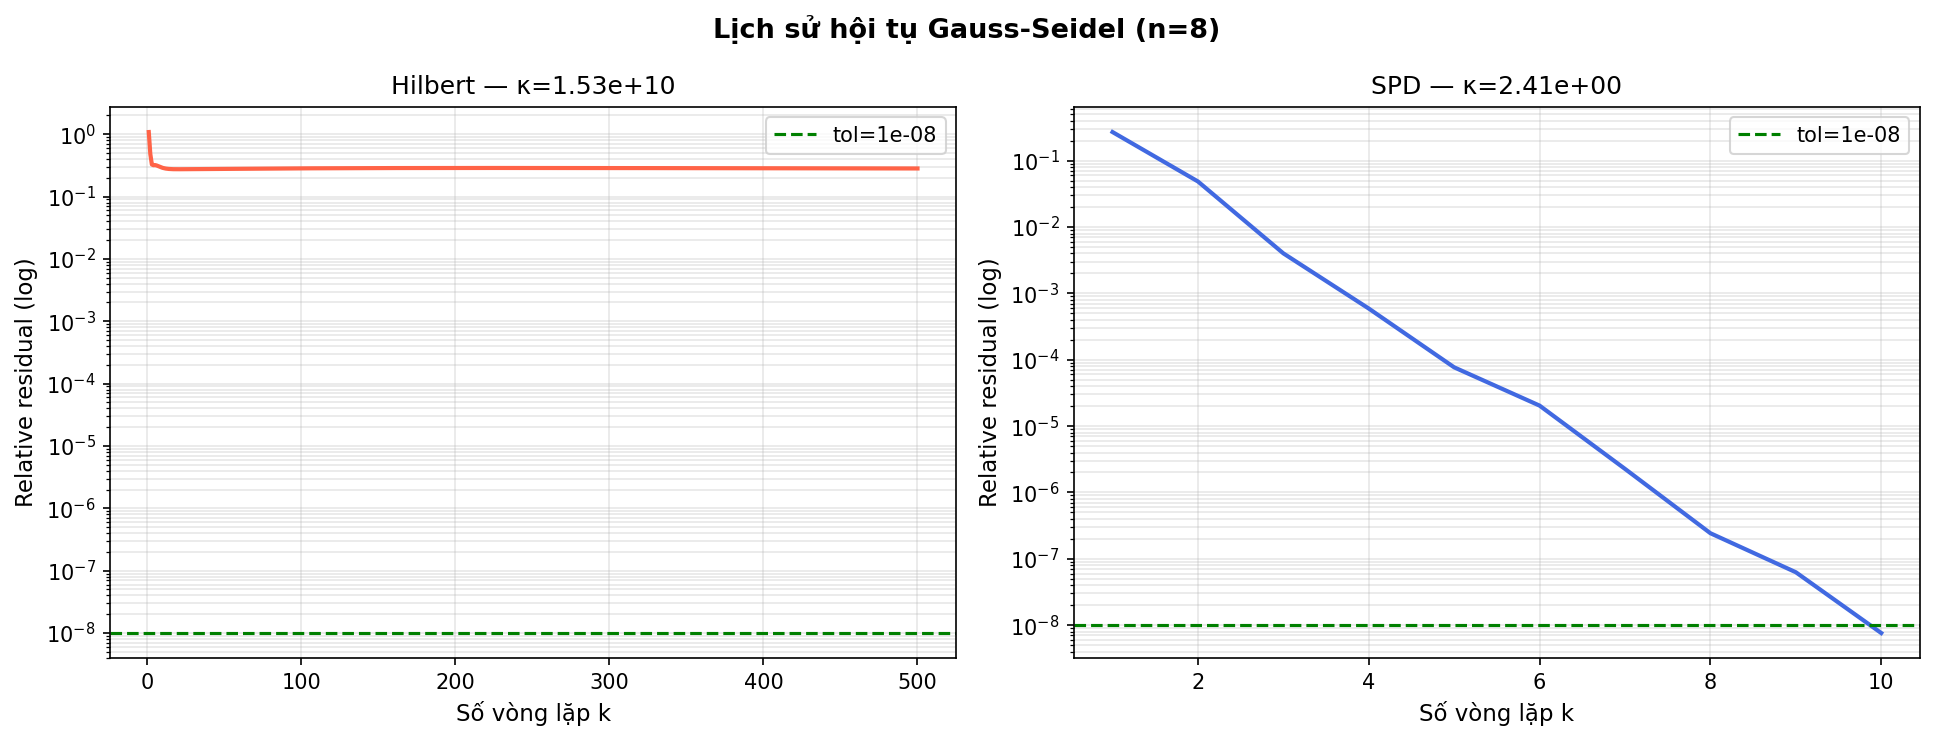
\includegraphics[width=0.9\textwidth]{../part3/fig3_convergence.png}
\caption{Hành vi hội tụ của phương pháp Gauss-Seidel trên hai loại ma trận.}
\label{fig:convergence}
\end{figure}

Trong tình huống bế tắc này, phương pháp Phân rã giá trị kỳ dị (SVD) nổi lên như giải pháp tối ưu và duy nhất có khả năng đối phó. Bằng cách tính toán nghiệm thông qua giả nghịch đảo Moore-Penrose:
\begin{equation}
    \mat{x} = \mat{V} \boldsymbol{\Sigma}^+ \mat{U}^T \mat{b}
\end{equation}
thuật toán SVD cho phép chúng ta áp dụng một ngưỡng (\textit{tolerance}) để chủ động loại bỏ các giá trị kỳ dị $\sigma_i$ quá nhỏ (gần $0$). Việc cắt tỉa này thực chất là loại bỏ các thành phần nhiễu đang khuếch đại sai số, giúp khôi phục lại tính ổn định cho nghiệm, biến SVD thành lựa chọn duy nhất mang lại kết quả đáng tin cậy~\cite{trefethen1997, golub2013, hansen1987}.

\subsection{Phân Tích Đánh Giá Trên Ma Trận Ngẫu Nhiên SPD (Well-conditioned)}

\subsubsection{Cơ Sở Toán Học và Đặc Điểm}

Trái ngược với sự bất ổn của ma trận Hilbert, báo cáo cũng xem xét nhóm ma trận đối xứng xác định dương được thiết kế đặc biệt để có tính chất well-conditioned. Các ma trận này được sinh ngẫu nhiên nhưng kiểm soát chặt chẽ phổ giá trị riêng thông qua công thức:
\begin{equation}
    \mat{A} = \mat{B}^T \mat{B} + \alpha \mat{I}
\end{equation}
trong đó $\mat{B}$ là một ma trận ngẫu nhiên đều và $\alpha > 0$ là tham số điều chỉnh độ bù đường chéo (\textit{diagonal shift}). Việc cộng thêm ma trận đường chéo $\alpha \mat{I}$ thực chất là tịnh tiến toàn bộ phổ giá trị riêng của hệ thống lên một lượng $\alpha$. Điều này đảm bảo rằng tất cả các giá trị riêng đều lớn hơn hẳn $0$, triệt tiêu hoàn toàn sự hiện diện của các thành phần kỳ dị. Nhờ đó, tỷ số giữa giá trị riêng cực đại và cực tiểu được giữ ở mức thấp (điển hình $\kappa(\mat{A}) \approx 10^1 \sim 10^3$), duy trì số điều kiện ở trạng thái lý tưởng, tạo ra một bài toán cực kỳ ổn định~\cite{trefethen1997}.

\subsubsection{Phân Tích Độ Tin Cậy và Hiệu Năng Của Các Thuật Toán}

Sự khác biệt về hiệu quả giữa các thuật toán trở nên hoàn toàn trái ngược khi áp dụng lên ma trận ngẫu nhiên SPD. Phương pháp khử Gauss tận dụng tối đa lợi thế của các phần tử trên đường chéo lớn. Quá trình chọn pivot diễn ra suôn sẻ, không gặp phải phép chia cho số nhỏ, dẫn đến nghiệm được giải mã với tốc độ chớp nhoáng và độ chính xác đạt đến giới hạn phần cứng ($\sim 10^{-16}$). Tương tự, phương pháp Gauss-Seidel tìm thấy môi trường hoàn hảo: tính xác định dương và các giá trị trên đường chéo đủ lớn đảm bảo cho dãy xấp xỉ thỏa mãn điều kiện hội tụ cực mạnh, hội tụ chỉ sau một số ít vòng lặp, đưa ra nghiệm xuất sắc trong thời gian ngắn nhất (như minh họa ở Hình~\ref{fig:time_complexity}).

Phương pháp phân rã QR vẫn duy trì phẩm chất ổn định tuyệt vời của mình, trả về nghiệm với sai số số học không đáng kể. Tuy nhiên, khi hệ thống vốn đã ổn định, sự phức tạp trong việc thiết lập các biến đổi Householder khiến nó tỏ ra chậm chạp hơn so với thuật toán Gauss thuần túy.

Đáng chú ý nhất là phương pháp SVD. Dù vẫn trả về nghiệm có độ chính xác hoàn hảo nhất, SVD lại bộc lộ nhược điểm trí mạng về chi phí tính toán (\textit{computational cost}). Trong một bài toán well-conditioned, việc tính toán toàn bộ phổ giá trị kỳ dị là thừa thãi và vô cùng tốn kém thời gian. Do đó, SVD không được khuyến nghị sử dụng thực tế cho lớp ma trận ngẫu nhiên này.

\subsection{Tổng Kết Sự So Sánh}

Bảng~\ref{tab:comparison_matrices_detailed} tổng hợp lại một cách chi tiết những quan sát và đánh giá đối với hai trường hợp ma trận đã nghiên cứu (Ma trận Hilbert và Ma trận Ngẫu nhiên SPD). Qua đó có thể thấy rõ sự phụ thuộc mật thiết giữa bản chất của ma trận và hiệu năng của từng thuật toán giải số.

\begin{table}[H]
\centering
\caption{Đối chiếu toàn diện đặc tính và kết quả giải số giữa hai họ ma trận}
\label{tab:comparison_matrices_detailed}
\renewcommand{\arraystretch}{1.4}
\setlength{\tabcolsep}{12pt}
\begin{tabular}{p{3.5cm}p{5cm}p{5cm}}
\toprule
\textbf{Tiêu chí đánh giá} & \textbf{Hệ Ma Trận Hilbert} & \textbf{Hệ Ma Trận Ngẫu nhiên SPD} \\
\midrule
\textbf{Bản chất điều kiện} & Ill-conditioned ($\kappa(\mat{A})$ khổng lồ) & Well-conditioned ($\kappa(\mat{A})$ nhỏ) \\
\textbf{Khả năng kháng nhiễu} & Cực kỳ mẫn cảm, mất mát thông tin & Ổn định, bảo toàn độ chính xác \\
\textbf{Phần dư (\textit{Residual})} & Nhỏ (gây ảo giác về độ chính xác) & Nhỏ và phản ánh đúng sai số thực \\
\textbf{Phương pháp Gauss} & Tích lũy sai số lớn, nghiệm sai lệch & Hoạt động hoàn hảo, tốc độ cao \\
\textbf{Khả năng lặp (Seidel)} & Phân kỳ hoặc trì trệ vô hạn & Hội tụ mạnh mẽ và nhanh chóng \\
\textbf{Vai trò của SVD} & Là giải pháp cứu cánh duy nhất & Quá tốn kém, không cần thiết \\
\bottomrule
\end{tabular}
\end{table}

\subsection{Phân Tích và Kết Luận}

Thông qua việc khảo sát các hiện tượng trên, chúng ta có thể đúc kết được những nguyên lý cốt lõi, mang tính nền tảng cho lĩnh vực Đại số Tuyến tính Số (\textit{Numerical Linear Algebra}).

\paragraph*{Khác Biệt Giữa Tính Ổn Định Của Thuật Toán và Độ Chính Xác Của Nghiệm.}
Một thuật toán được chứng minh là ổn định về mặt số học (như phân rã QR Householder) hoàn toàn không đảm bảo rằng nó sẽ luôn trả về một nghiệm chính xác. Thuật toán ổn định chỉ có nghĩa là nó không tự sinh ra thêm lượng sai số quá mức trong quá trình tính toán. Tuy nhiên, nếu bản thân bài toán vốn dĩ đã là ill-conditioned, bản chất toán học của hệ thống sẽ tự khuếch đại những sai số ban đầu, khiến mọi thuật toán dù tốt đến đâu cũng đành bất lực trong việc tìm ra nghiệm đúng~\cite{trefethen1997, higham2002, wilkinson1965}.

\paragraph*{Conditioning Là Đặc Tính Bền Vững.}
Số điều kiện là DNA của ma trận. Chúng ta không thể cải thiện sự tồi tệ của một bài toán ill-conditioned chỉ đơn thuần bằng cách thay thế thuật toán giải từ Gauss sang QR. Để đối phó với nó, bắt buộc phải can thiệp vào bản chất không gian số, chẳng hạn như sử dụng hệ thống số với độ chính xác cao hơn (\textit{quadruple precision}), hoặc áp dụng các kỹ thuật chính quy hóa (\textit{regularization}) như Tikhonov, hoặc sử dụng cơ chế cắt tỉa giá trị kỳ dị thông qua SVD để thiết lập lại một bài toán xấp xỉ nhưng ổn định hơn~\cite{golub2013}.

\paragraph*{Sự Cần Thiết Của Đánh Giá Đa Chiều.}
Việc đánh giá sự thành công của một mô hình giải số không thể chỉ dừng lại ở chỉ số phần dư $\norm{\mat{A}\mat{x} - \mat{b}}_2$. Đối với các hệ thống phức tạp, người kỹ sư bắt buộc phải trang bị các công cụ chẩn đoán bổ sung, bao gồm việc xấp xỉ số điều kiện $\kappa(\mat{A})$ và kiểm soát sai số tương đối (\textit{relative error}) để tránh rơi vào cạm bẫy của những phần dư giả mạo~\cite{demmel1997}.

\paragraph*{Lựa Chọn Thuật Toán Phù Hợp.}
Không có một thuật toán nào là tối ưu cho mọi trường hợp. Khi ma trận đảm bảo tính xác định dương và ổn định, ưu tiên cao nhất là tốc độ, các phương pháp như Cholesky hay Gauss là lựa chọn hàng đầu. Khi đối mặt với hệ thống tổng quát có rủi ro tiềm ẩn, phương pháp phân rã QR đem lại sự an tâm về độ bền vững số học. Và cuối cùng, khi chạm trán với những bài toán ill-conditioned thực sự, SVD là công cụ giải phẫu duy nhất đủ khả năng cắt bỏ các thành phần nhiễu để cứu vãn hệ thống.

\subsection{Kết Luận}

Tóm lại, thực nghiệm với hai họ ma trận Hilbert và Ngẫu nhiên SPD đã phơi bày hai thái cực đối lập trong tính toán số học. Ma trận Hilbert là đại diện tiêu biểu cho sự sụp đổ của các phương pháp giải số truyền thống trước rào cản ill-conditioned, nơi mà chỉ có những công cụ phân tích sâu sắc như SVD mới có thể khôi phục lại trật tự. Ở chiều ngược lại, họ ma trận Ngẫu nhiên SPD được kiểm soát phổ chứng minh rằng một bài toán được thiết lập tốt (well-posed) sẽ là nền tảng để mọi thuật toán giải số có thể phô diễn tối đa tốc độ và sự chính xác của mình. Đồ thị thời gian cũng củng cố mạnh mẽ sự đánh đổi thiết yếu giữa độ phức tạp tính toán và độ tin cậy của nghiệm.

\begin{note}[Triết lý tối thượng của Numerical Linear Algebra]
Trong thực tiễn tính toán khoa học, \textbf{chất lượng của bài toán được đặt ra luôn có tầm quan trọng vượt xa sự tinh vi của thuật toán được sử dụng để giải nó}. Nhiệm vụ quan trọng nhất không phải là tìm ra một thuật toán hoàn hảo cho một bài toán tồi, mà là nghệ thuật biến đổi (\textit{preconditioning}) để đưa một bài toán tồi về trạng thái well-conditioned, nơi mà những thuật toán đơn giản nhất cũng có thể tỏa sáng~\cite{trefethen1997}.
\end{note}
